\chapter{Gęste sieci neuronowe}
\label{chap:siecifc}

\section{Algorytmy uczące się}

W przypadku każdego wariantu sieci neuronowej mówimy o modelu luźno inspirowanym biologicznym odpowiednikiem. Jego zadaniem jest rozwiązanie pewnej zadanej klasy problemu \(T\). Proces ten nazywamy nauką lub treningiem. Nauka została zdefiniowana przez prof. Toma Mitchella w następujący sposób:
\textit{,,Program komputerowy uczy się na podstawie doświadczenia \(E\), w związku z pewną klasą problemów \(T\) przy uwzględnieniu miary skuteczności \(P\), jeżeli jego sprawność w wykonywaniu zadań \(T\), wyrażona przy pomocy \(P\)
rośnie razem z doświadczeniem \(E\).''}

Proces treningu w przypadku modeli przytoczonych w tej pracy będzie polegał na ustaleniu wag przy poszczególnych węzłach sieci neuronowej, dalej nazwanych neuronami. Składać się on będzie z dwóch części: propagacji w przód oraz propagacji wstecznej. 

Praca traktuje o zagadnieniach z dziedziny uczenia z nauczycielem (ang. \textit{Supervised Learning}). W związku z tym, podczas treningu, propagacja w przód będzie polegała na obliczeniu wartości poprzez sieć dla danych uprzednio sklasyfikowanych i oznakowanych przy pomocy innego automatu lub człowieka.
Uzyskany wynik jest początkowo losowy i zostaje użyty do obliczenia wartości funkcji kosztu, opisanych w rozdziale \ref{sec:costfunction}.
Na podstawie funkcji kosztu, wagi sieci zostaną skorygowane w procesie propagacji wstecznej.

\section{Gęsta sieć neuronowa}

Podstawową implementacją sieci neuronowej jest tzw. sieć w pełni połączona (ang. \textit{Fully Connected Network}). Składa się z warstw: wejściowej, jednej lub więcej warstw ukrytych i warstwy wyjściowej.  

\begin{figure}[ht]
\centerline{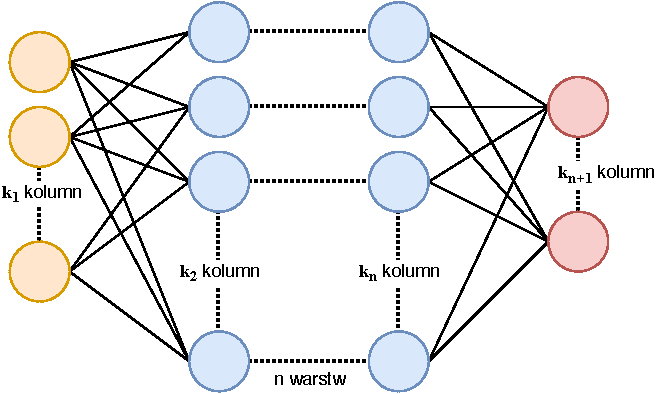
\includegraphics[scale=0.9]{resources/fc/fully_connected.pdf}}
\caption{Schemat w pełni połączonej sieci neuronowej.}
\label{fig:schematFc}
\end{figure}

W przypadku, gdy model zawiera stosunkowo dużą liczbę warstw ukrytych, na schemacie oznaczonych jako n, mówimy o głębokich sieciach neuronowych. 
Ten wariant sieci neuronowej charakteryzuje się tym, że każdy węzeł jej warstwy jest połączony z każdym. Warstwa wejściowa, oznaczona kolorem żółtym, doprowadza dane wejściowe do warstw ukrytych oznaczonych kolorem niebieskim. Warstwa wyjściowa oznaczona jest kolorem czerwonym.

\section{Neuron gęstej sieci neuronowej}
Pojedynczy neuron można przedstawić następującym schematem \ref{fig:neuronFc}.

\begin{figure}[ht]
\centerline{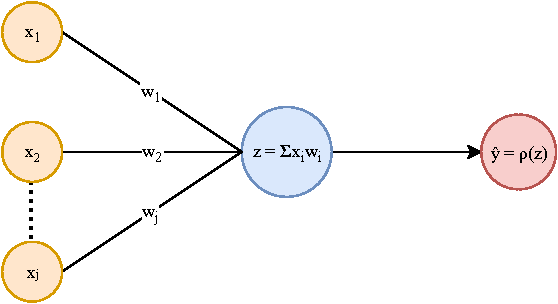
\includegraphics[scale=1]{resources/fc/single_neuron_fc.pdf}}
\caption{Schemat w pełni połączonej sieci neuronowej.}
\label{fig:neuronFc}
\end{figure}

Wartości \(a_1\) do \(a_j\) reprezentują wartości z warstwy sieci neuronowej, a w szczególności wartości początkowe \(x_1 ... x_j\). Każda z nich jest przemnożona przez odpowiadającą jej wagę \(w\) i zsumowana. Następnie, tak uzyskaną wartość używamy do wyliczenia \(\rho\) nazwanego funkcją aktywacji neuronu. Zadaniem \(\rho\) jest wprowadzenie elementu nieliniowości. Mniej formalnie, ma na celu ustalenie czy neuron powinien zostać aktywowany czy też nie.
Najpopularniejsze funkcje aktywacji przedstawia rysunek \ref{fig:activations}.

\begin{figure}
\subfloat[Funkcja \textit{ReLU}.]{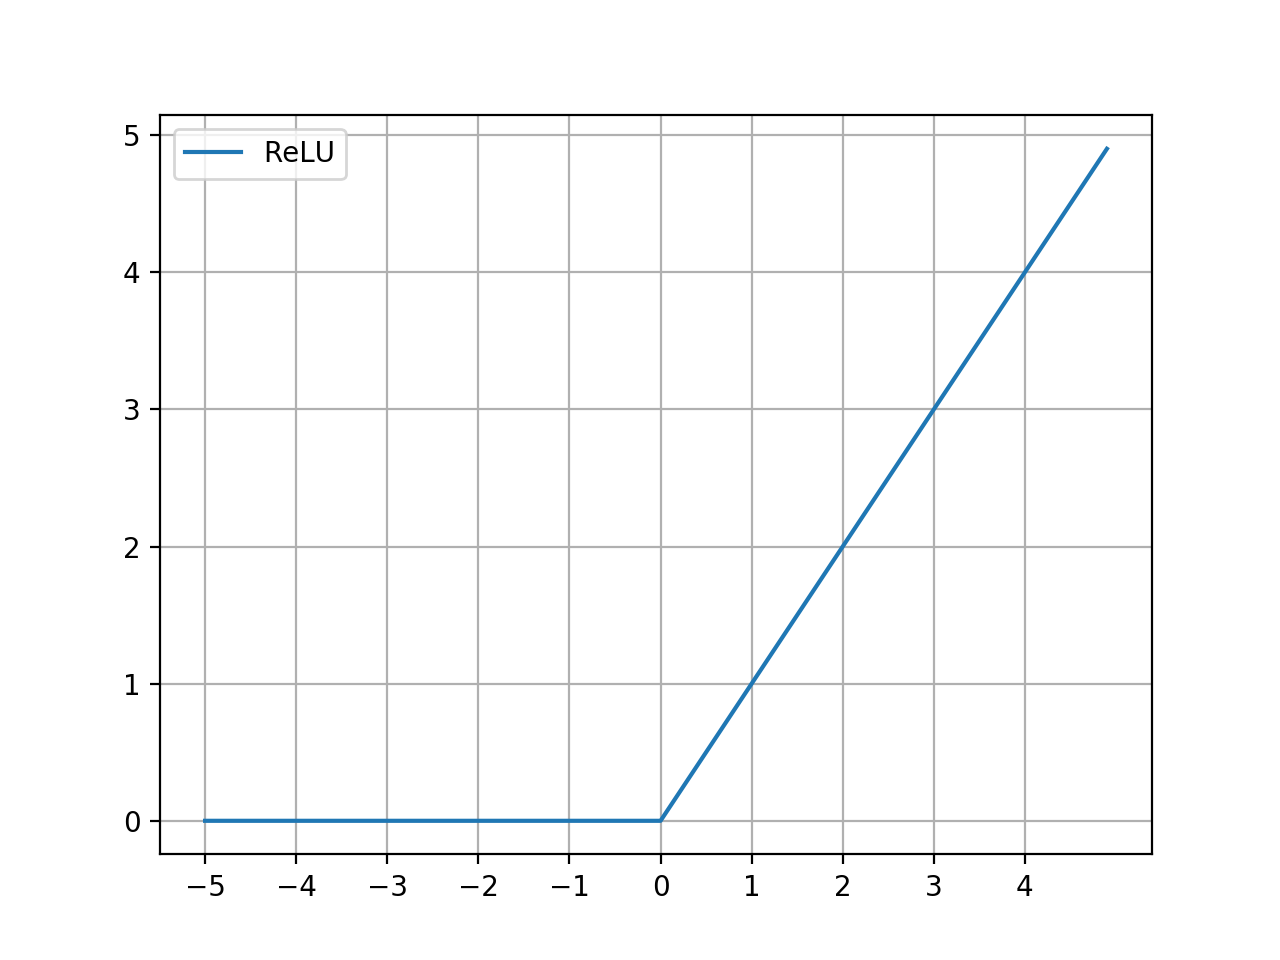
\includegraphics[width = 2in]{resources/fc/relu.png}} 
~
\subfloat[Funkcja \textit{Sigmoid}.]{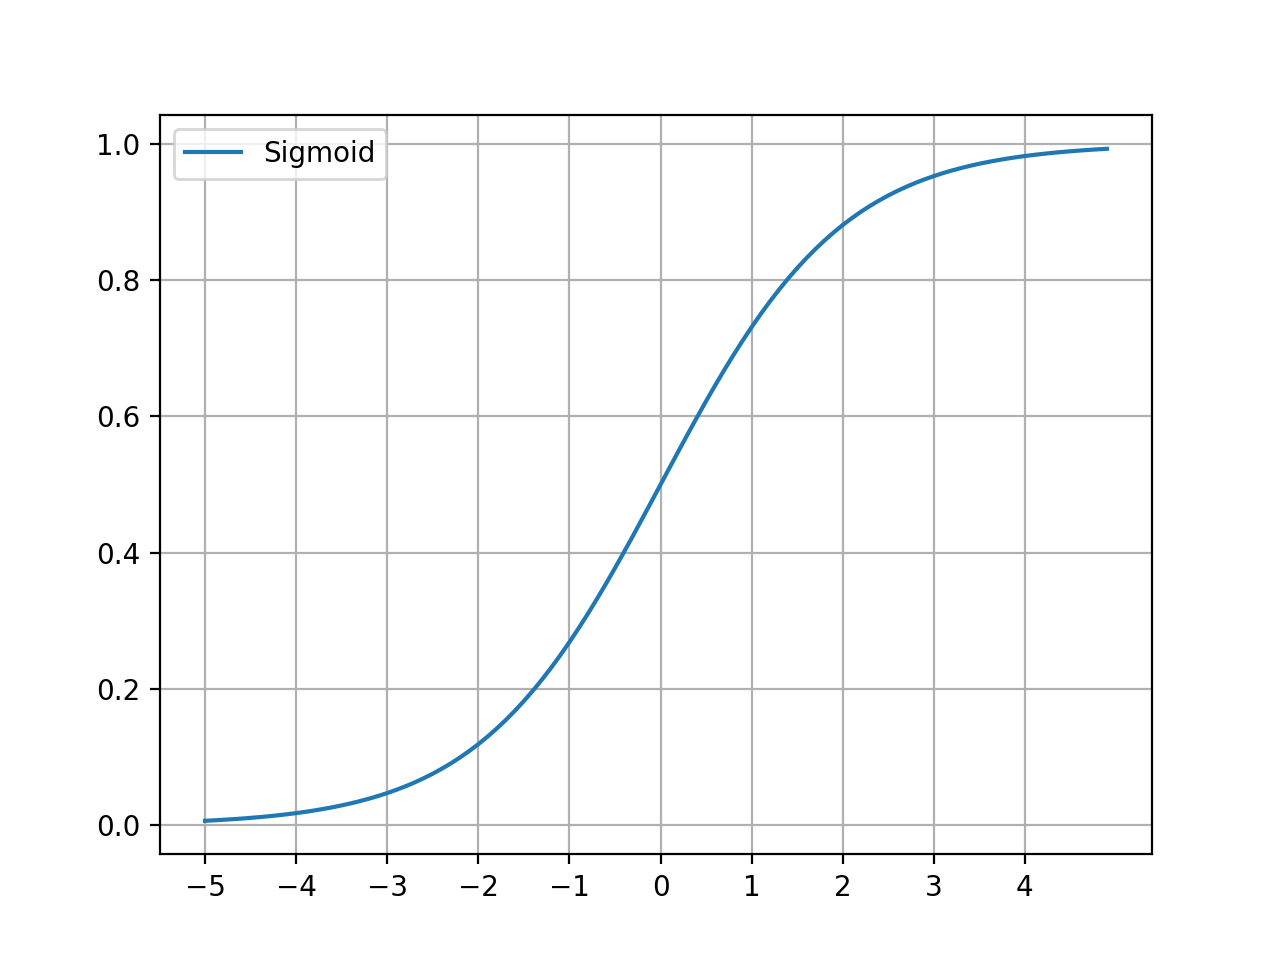
\includegraphics[width = 2in]{resources/fc/sigmoid.png}} 
~
\subfloat[Funkcja \textit{tangens hiperboliczny}.]{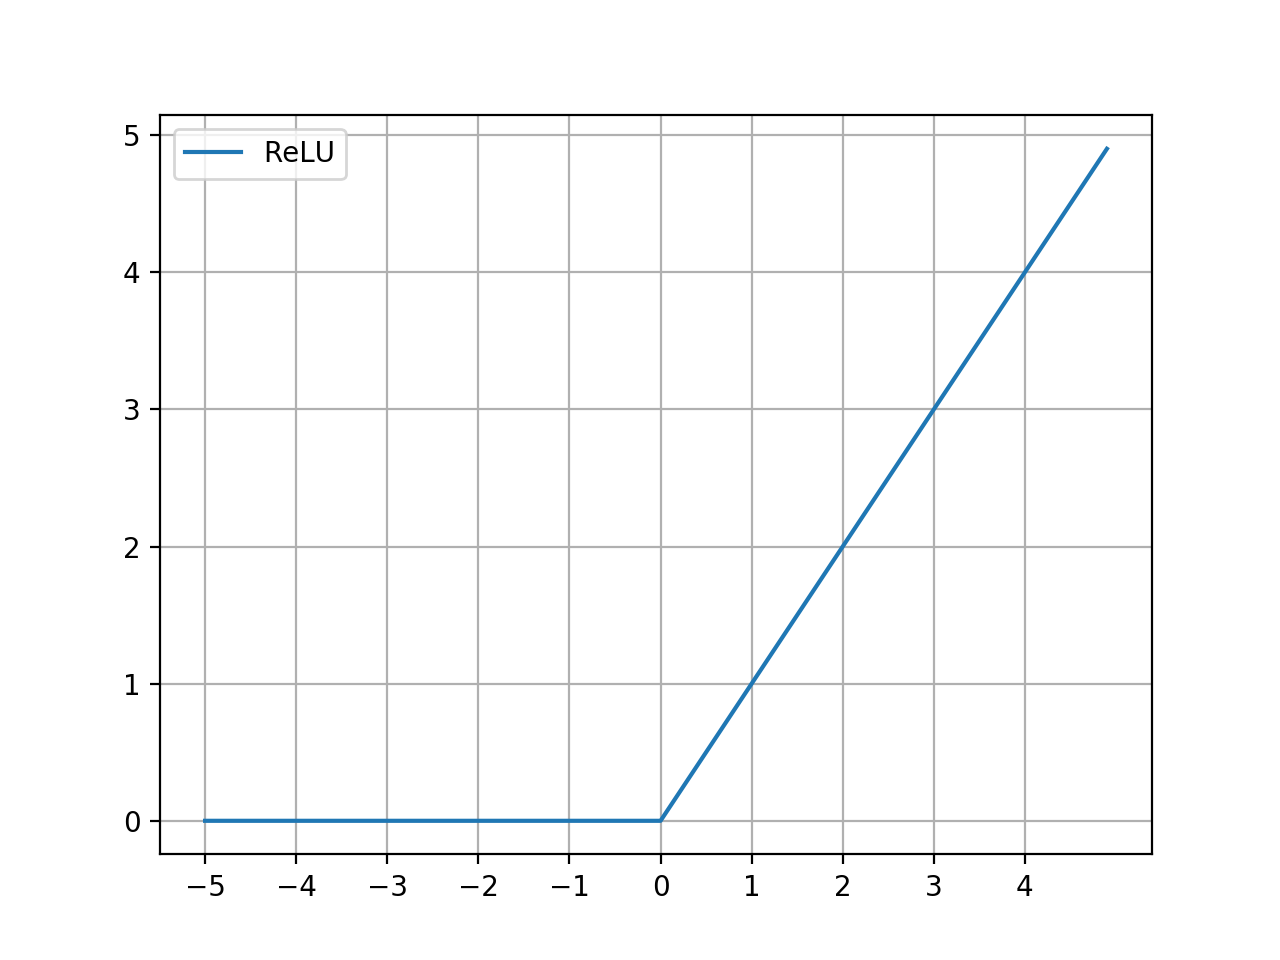
\includegraphics[width = 2in]{resources/fc/relu.png}} 
\caption{Wybrane funkcje aktywacji.}
\label{fig:activations}
\end{figure}

\section{Propagacja w przód}

By ustalić wartość neuronu, posługujemy się następującym wzorami:

\[z_{n}^{\lbrack l\rbrack}=\sum_{i=1}^{j}{w_{\text{ni}}^{\lbrack l\rbrack}a_{i}^{\lbrack l - 1\rbrack} + b_{n}^{\lbrack l\rbrack}},\]

\[a_{n}^{\lbrack l\rbrack}=\rho(z_{n}^{\lbrack l\rbrack}),\]

Gdzie:
\begin{itemize}
\item \(\rho\) to funkcja aktywacji,
\item \textsubscript{(n)} oznacza numer neuronu w warstwie,
\item \textsuperscript{{[}l{]}} to numer warstwy,
\item \(b\) to tak zwany bias. Jego wartość jest ustalana razem z wagami w procesie propagacji wstecznej,
\item \(w_{\text{ni}}^{\lbrack l\rbrack}\) jest to \textbf{i}-ta waga neuronu numer \textbf{n}, warstwy \textbf{l},
\item \(a_{i}^{\lbrack l - 1\rbrack}\) jest to wartość \textbf{i}-tego neuronu warstwy \({[}l-1{]}\), w szczególnym przypadku może być to jedna z wartości wejściowych \(x\).
\end{itemize}

Używając tych wzorów, możemy obliczać wartości wag kolejnych warstw sieci aż do warstwy ostatniej.
Tam, w zależności od postawionego problemu, możemy wyliczyć kolejne aktywacje przy pomocy \(\rho\) (tylko w odróżnieniu od warstw ukrytych nie stosuje się tam \(ReLU\), tylko np. \(sigmoid\) lub możemy użyć funkcji \(softmax\):

\[S(y_{i}) = \frac{e^{y_{\text{i\ }}}}{\sum_{j}^{y_{n}}e^{y_{j}}}\]

Jest to funkcja, która przyjmuje \(y_{n}\) elementowy wektor składający się z liczb rzeczywistych i przeprowadza go w rozkład prawdopodobieństwa składającego się z \(y_{n}\) elementów. Przydatną jej cechą jest to, że zachowuje proporcjonalny udział wartości w wynikowym prawdopodobieństwie -- tj. elementy o wyższej wartości mają przypisane wyższe wartości prawdopodobieństwa.

Na przykładzie klasyfikacji, by uzyskać wynik, który można zinterpretować, należy posłużyć się następującym sposobem postępowania. Niech przedostatnia warstwa \(a^{\lbrack L - 1\rbrack}\) sieci posiada \(n\) węzłów, których liczba jest równa liczbie klas rzeczy, które chcemy rozpoznawać. Przyjmijmy również, że dana rzecz nie może należeć do dwóch klas równocześnie.

W przypadku aktywacji przy pomocy sigmoid uzyskujemy algorytm nazywany ,,jeden kontra każdy'' (ang. \textit{one vs all}). Każdy z węzłów \(a_{i}^{\left\lbrack L - 1 \right\rbrack}\) jest wejściem dla \(\rho\). Po wyliczeniu wartości, przyjmujemy próg z przedziału \({[}0, 1{]}\), by uzyskać wynik dla każdego neuronu z osobna.

\begin{figure}[ht]
\centerline{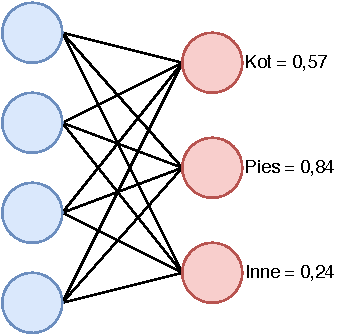
\includegraphics[scale=1]{resources/fc/sigmoid_1vsAll.pdf}}
\caption{Przykładowy wynik \textit{1 vs all} dla trzech klas ze zbioru \big\{Kot, Pies, Inne.\big\}}
\label{fig:1v_all}
\end{figure}

By zobrazować działanie algorytmu posłużę się przykładem. Załóżmy, że zbudowano klasyfikator, mający na celu przypisanie danej postaci klasy ze zbioru {kot, pies, inne}. Każdą aktywację z warstwy \(L-1\) przeprowadzamy z osobna, przy pomocy \(sigmoid\) w wartość z przedziału od 0 do 1. Następnie, przyjmujemy próg, powyżej którego mówimy, że sieć rozpoznała daną klasę. Przykładowo, w przypadku z rysunku \ref{fig:1v_all} przyjmując próg równy 0.5 mamy dwa możliwe wyniki. By wyeliminować jeden z nich możemy zwiększyć próg do 0.6 lub wybrać neuron z wyższą wartością. W obu przypadkach będzie to neuron oznaczający to, że klasyfikator rozpoznał psa.

\begin{figure}[ht]
\centerline{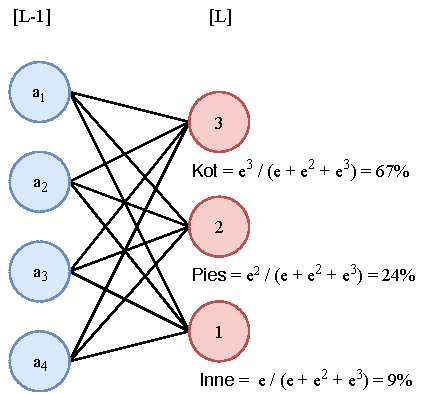
\includegraphics[scale=1]{resources/fc/softmax_fc.pdf}}
\caption{Przykładowy wynik z użyciem \textit{softmax}.}
\label{fig:softmax}
\end{figure}

Istnieją inne metody aktywacji warstw wyjściowych. Każda z nich, która zostanie użyta w tej pracy będzie trzymała się podobnego schematu. Wynikiem sieci gęsto połączonej będzie wektor zer i jedynek, w którym 1 ustawione na odpowiednim miejscu w rzędzie będzie oznaczało, że dany przedmiot został rozpoznany. W przypadku rozrysowanym na rysunku \ref{fig:softmax} będzie to wektor \([1 0 0]\).

\section{Funkcja kosztu}
\label{sec:costfunction}

W przypadku problemów poruszanych w tej pracy, funkcję kosztu należy rozumieć jako przyporządkowanie wynikom uzyskanym przy pomocy sieci neuronowej wraz ze znanymi poprawnymi odpowiedziami, liczby reprezentującej „koszt”. Wartość kosztu należy interpretować jako skuteczność w odgadywaniu poprawnych wyników w taki sposób, że im niższy koszt tym wyższa poprawność predykcji. Można powiedzieć, że sieć neuronowa próbuje znaleźć najwierniejsze przybliżenie oryginalnej, nieznanej funkcji nazywanej hipotezą, a celem funkcji kosztu jest modelowanie różnicy między przybliżeniem a funkcją, której próbujemy nauczyć sieć.

Istnieje wiele różnych funkcji kosztu. Opiszę tutaj tylko funkcję \textit{cross entropy loss}, która jest często wybierana przy treningu sieci, które na ostatniej warstwie używają \(softmax\).

\[J(w) = \frac{1}{m}\ \sum_{i = 1}^{m}{\lbrack y_{i}\log{\acute{y}_{i} + \left( 1 - y_{i} \right)\log{(1 - \ \acute{y}_{i})}}\rbrack},\]

gdzie:

\begin{itemize}
\item
  \(w\) -- wagi sieci neuronowej,
\item
  \(m\) -- liczba klasyfikowanych przykładów,
\item
  \(y_{i}\) -- wartość oczekiwana dla przykładu numer i
\item
    \(\acute{y}_{i}\) -- wartość uzyskana przy pomocy sieci dla przykładu numer \(i\).
\end{itemize}

Jest to suma błędów pojedynczych predykcji dla wszystkich przykładów dostępnych w danym zestawie danych treningowych. Zadaniem treningu, będzie znalezienie jej minimum dla danego problemu.
By udało się to sprawnie zrobić, będę korzystał z faktu, że ta i inne funkcje kosztu, którymi będę się posługiwał są różniczkowalne i ciągłe.

\section{Propagacja wstecz}
\label{sec:backprob}

Jest to modyfikacja wag sieci neuronowej \(w\) z uwzględnieniem funkcji kosztu \(J(w)\). Popularnym sposobem jest metoda gradientu prostego (częściej spotykana w wariacji z tzw. pędem, z angielskiego \textit{Gradient descent with momentum} lub dalsze jej modyfikacje jak np. algorytm
\textit{Adaptive moment estimation}, znany jako \textit{Adam}). W swej najprostszej wersji można sprowadzić go do następujących kroków:

\begin{enumerate}
\def\labelenumi{\arabic{enumi}.}
\item
  Wybierz punkt startowy \(w_{0}\).
\item
  \(w_{k + 1} = w_{k} - \alpha\ \nabla f(w_{k})\).
\item
  Jeżeli \(\left\| w_{k + 1} - w_{k} \right\|\  \geq \varepsilon\) idź
  do 2.
\item
  Koniec.
\end{enumerate}

gdzie:

\begin{itemize}
\item
  \(\alpha\) -- współczynnik uczenia: zazwyczaj niewielka
  (\(\alpha\  < 0.01)\) dodatnia liczba rzeczywista. Podczas treningu
  sieci neuronowych często \(\alpha = const\), choć sam algorytm
  gradientu prostego posiada wariację ze zmienną wartością \(\alpha\).
\item
  \(\nabla f(w_{k})\) -- jest to gradient funkcji reprezentującej
  funkcję przybliżającą hipotezę.
\item
  \(w\) -- wagi sieci,
\item
  \(\varepsilon\) -- niewielka wartość będąca kryterium stopu dla
  algorytmu. Wykorzystuje fakt, że różnice w wartości wag będą maleć
  wraz ze zbliżaniem się do minimum funkcji \(J(w)\).
\end{itemize}

Krok pierwszy, czyli wybranie punktu startowego jest rozwiązany przy pomocy losowej inicjalizacji wag \(w\). Często stosuje się tu różne heurystyki dostosowane do użytej funkcji aktywacji (dla \(\tanh\) jest to przykładowo inicjalizacja \(Xaviera\).

Kłopotliwym zagadnieniem może wydawać się wyliczenie gradientu \(\nabla f(w)\). Nie posiadając formalnej definicji hipotezy, tylko jej aproksymację w postaci sieci neuronowej musimy, posłużyć się funkcją kosztu \(J(w)\) i zależnością:

gdy:

\[J\left( z \right) = J(a\left( z \right))\]

to:

\[\frac{dJ}{dz} = \frac{dJ}{da} \frac{da}{dz}\]

Posługując się nimi, możemy wyjść od wzoru funkcji kosztu \(J(w)\) i na tej podstawie aktualizować wartość wag ostatniej warstwy. Co więcej, możemy przy pomocy nowo wyliczonych wag, wyliczyć nowe wartości wag warstwy przedostatniej i tak niejako licząc warstwa po warstwie, aktualizować wszystkie wagi sieci neuronowej.

Niestety konkretne wzory służące do aktualizacji wag muszą być wyprowadzone dla każdej z funkcji kosztu z osobna. Całe szczęście biblioteki do uczenia maszynowego mają zaimplementowane większość z nich w taki sposób, że użytkownik musi tylko zaimplementować propagację w przód i wybrać funkcję kosztu. Nie mniej jednak, by zobrazować ten proces wyprowadzę wzory potrzebne dla propagacji wstecznej dla dwuwarstwowej sieci neuronowej. Propagację na dalsze warstwy będą tylko ponownym wykorzystaniem
tych samych wzorów w zastosowaniu do kolejnych wag.

Schemat sieci neuronowej wykorzystanej do obliczeń znajduje się na rysunku \ref{fig:backprop_fc}.

\begin{figure}[ht]
\centerline{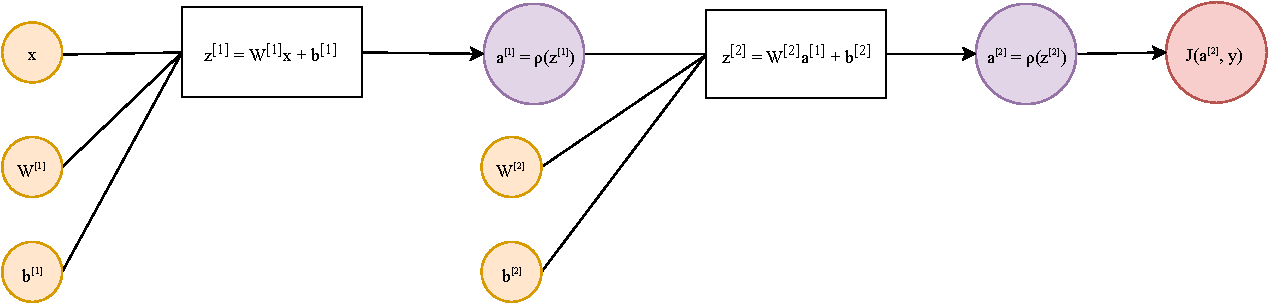
\includegraphics[scale=0.7]{resources/fc/backprop_fc_cross_entropy.pdf}}
\caption{Przykładowy schemat sieci neuronowej, przy liczeniu propagacji
wstecznej.}
\label{fig:backprop_fc}
\end{figure}

Dla pojedynczego przykładu ze zbioru treningowego:

\[J\left( w \right) = y\log{a(w)^{\lbrack 2\rbrack} + \left( 1 - y \right)\log{(1 - \ a(w)^{\lbrack 2\rbrack})}}\]

oraz przyjmując \(sigmoid\) za funkcję aktywacji:

\[\rho = \frac{e^{z}}{e^{z}\  + \ 1},\]

wtedy:

\begin{enumerate}
\def\labelenumi{\arabic{enumi}.}
\item
  \(\frac{dJ}{da^{\left\lbrack 2 \right\rbrack}} = - \frac{y}{a^{\lbrack 2\rbrack}} + \frac{1 - y}{1 - a^{\lbrack 2\rbrack}},\)
\item
    \(\frac{da^{\left\lbrack 2 \right\rbrack}}{dz^{\lbrack 2\rbrack}} = \frac{d\rho^{\lbrack 2\rbrack}}{dz} = \frac{e^{z^{\left\lbrack 2 \right\rbrack}}}{\left( 1\  + {\ e}^{z^{\left\lbrack 2 \right\rbrack}} \right)^{2}} = \frac{e^{-z^{\left\lbrack 2 \right\rbrack}}}{\left( 1\  + {\ e}^{-z^{\left\lbrack 2 \right\rbrack}} \right)^{2}} = \frac{1}{1\  + {\ e}^{- z^{\lbrack 2\rbrack}}} \frac{1\  + \ \left( e^{- z^{\left\lbrack 2 \right\rbrack}} \right)\ \  - \ 1}{\left( 1\  + {\ e}^{- z^{\left\lbrack 2 \right\rbrack}} \right)} = \frac{1}{1\  + {\ e}^{- z^{\left\lbrack 2 \right\rbrack}}} (1 - \frac{1}{\left( 1\  + {\ e}^{- z^{\left\lbrack 2 \right\rbrack}} \right)}) = a^{\lbrack 2\rbrack}(1 - a^{\left\lbrack 2 \right\rbrack})\),
\item
  \(\frac{dJ}{dz^{\left\lbrack 2 \right\rbrack}} = \frac{dJ}{da^{\left\lbrack 2 \right\rbrack}} \frac{da^{\left\lbrack 2 \right\rbrack}}
  {dz^{\left\lbrack 2 \right\rbrack}} = \left\lbrack - \frac{y}{a^{\left\lbrack 2 \right\rbrack}} + \frac{1 - y}{1 - a^{\left\lbrack 2 \right\rbrack}}
  \right\rbrack a^{\left\lbrack 2 \right\rbrack}\left( 1 - a^{\left\lbrack 2 \right\rbrack} \right) = - \left\lbrack \frac{y\left( 1 - a^{\lbrack 2\rbrack} \right)\  + \ a^{\lbrack 2\rbrack}
  \left( 1 - y \right)}{a^{\lbrack 2\rbrack}\left( 1\ -\ a^{\lbrack 2\rbrack} \right)} \right\rbrack a^{\left\lbrack 2 \right\rbrack}
  \left( 1 - a^{\left\lbrack 2 \right\rbrack} \right) = \ a^{\left\lbrack 2 \right\rbrack} - y\).
\end{enumerate}

Dysponując \(\frac{dJ}{dz^{\left\lbrack 2 \right\rbrack}}\),
\(a^{\lbrack 2\rbrack}\) i \(a^{\lbrack 1\rbrack}\) (z fazy propagacji
w przód) możemy zaktualizować \(w^{\lbrack 2\rbrack}\) i
\(b^{\lbrack 2\rbrack}\),

\begin{enumerate}
\def\labelenumi{\arabic{enumi}.}
\setcounter{enumi}{3}
\item
  \(\frac{dJ}{dw^{\lbrack 2\rbrack}} = \frac{dJ}{dz^{\left\lbrack 2 \right\rbrack}} \frac{dz^{\left\lbrack 2 \right\rbrack}}{dw^{\left\lbrack 2 \right\rbrack}} = {(a}^{\left\lbrack 2 \right\rbrack} - y)a^{\lbrack 1\rbrack}\),
\item
  \(\frac{dJ}{db^{\lbrack 2\rbrack}} = \ \frac{dJ}{dz^{\left\lbrack 2 \right\rbrack}} \frac{dz^{\left\lbrack 2 \right\rbrack}}{db^{\left\lbrack 2 \right\rbrack}} = \ {(a}^{\left\lbrack 2 \right\rbrack} - y)\).
\end{enumerate}

Powyższe obliczenia pokazują, w jaki sposób obliczyć nową wartość wag między funkcją kosztu a ostatnią warstwą sieci. Kolejne kroki pokażą, w jaki sposób obliczyć nową wartość wag pomiędzy dwiema warstwami (można te kroki uogólniać na dowolną liczbę warstw).

\begin{enumerate}
\def\labelenumi{\arabic{enumi}.}
\setcounter{enumi}{5}
\item
  \(\frac{dJ}{da^{\lbrack 1\rbrack}} = \frac{dJ}{dz^{\lbrack 2\rbrack}} \frac{dz^{\left\lbrack 2 \right\rbrack}}{da^{\left\lbrack 1 \right\rbrack}} = {(a}^{\left\lbrack 2 \right\rbrack} - y) w^{\lbrack 2\rbrack},\)
\item
  \(\frac{dJ}{dz^{\left\lbrack 1 \right\rbrack}} = \frac{dJ}{da^{\left\lbrack 1 \right\rbrack}} \frac{da^{\left\lbrack 1 \right\rbrack}}{dz^{\left\lbrack 1 \right\rbrack}} = {w^{\left\lbrack 2 \right\rbrack}(a}^{\left\lbrack 2 \right\rbrack} - y){a}^{\left\lbrack 1 \right\rbrack}(1 - a^{\left\lbrack 1 \right\rbrack}).\)
\end{enumerate}

(\(\frac{da^{\left\lbrack 1 \right\rbrack}}{dz^{\left\lbrack 1 \right\rbrack}}\)
obliczone analogicznie jak w kroku numer. 2),

Stąd wiadomo jak obliczyć wagi \(w^{\left\lbrack 1 \right\rbrack}\ \)i
\(b^{\left\lbrack 1 \right\rbrack},\)

\begin{enumerate}
\def\labelenumi{\arabic{enumi}.}
\setcounter{enumi}{7}
\item
  \(\frac{dJ}{dw^{\lbrack 1\rbrack}} = \frac{dJ}{dz^{\lbrack 1\rbrack}} \frac{dz^{\left\lbrack 1 \right\rbrack}}{dw^{\left\lbrack 1 \right\rbrack}} = {w^{\left\lbrack 2 \right\rbrack}(a}^{\left\lbrack 2 \right\rbrack} - y){a}^{\left\lbrack 1 \right\rbrack}(1 - a^{\left\lbrack 1 \right\rbrack}) x,\)
\item
  \(\frac{dJ}{db^{\lbrack 1\rbrack}} = \frac{dJ}{dz^{\lbrack 1\rbrack}} \frac{dz^{\left\lbrack 1 \right\rbrack}}{dw^{\left\lbrack 1 \right\rbrack}} = {w^{\left\lbrack 2 \right\rbrack}(a}^{\left\lbrack 2 \right\rbrack} - y){a}^{\left\lbrack 1 \right\rbrack}(1 - a^{\left\lbrack 1 \right\rbrack}).\)
\end{enumerate}

Po takim cyklu, należy wybrać kolejny przykład z zestawu treningowego, przeliczyć propagację w przód, funkcję kosztu a następnie znów propagację w tył, aż kryterium stabilności metody gradientu prostego zostanie spełnione.

